\chapter{Experiments}
The main goal of this work was to use proximal policy optimization to simulate a parking situation in a virtual environment.

The tool used to create the simulation was Unity (version 2021.3.7f1), developed by Unity Technologies, commonly used as a game engine. All the assets used are available for free in the Unity Store.

Unity provides a open-source \textit{toolkit} called ML-Agents, which enables developers to create and train AI agents inside the platform. ML-Agents also provides its own implementation of proximal policy optimization, as described in \cite{schulman2017proximal}.

The first experiment is the simplest, where we keep every spawn fixed across all episodes. In the following experiments, we randomize the spawns of the agent, parking spot and obstacles (parked cars), until the environment is completely random.

\section{Hyperparameters and Evaluation Metrics}
In the context of machine learning, a \textit{hyperparameter} is a parameter whose value is used to control the learning process. The main difference of a hyperparameter and a parameter is that the values of hyperparameters are manually set, while parameters (for example, node weights in a neural network) are derived during training.

For the neural network, which will be used as an approximator for the policy, the hyperparameters to be set are the \textbf{number of hidden layers} and the \textbf{number of units per layer}, as seen in section \ref{sec:nn}.

For PPO, we need to set the \textbf{batch size}, \textbf{buffer size}, \textbf{divergence limit $\epsilon$}, \textbf{exponential weight discount $\lambda$}, \textbf{learning rate $\alpha$}, \textbf{number of epochs}, \textbf{time horizon} and \textbf{max step}.

\textbf{Batch size.} Determines how many experiences (trajectories) are used for each gradient descent update.

\textbf{Buffer size.} Determines how many experiences (trajectories) are collected before a gradient descent update is performed on them all.

\textbf{Epochs.} It is the number of passes through the experience buffer during gradient descent.

We update the model every time we get to a determined number of timesteps, determined by the buffer size. During this update, the buffer is divided into $n$-sized batches, determined by batch size, and a gradient descent update is performed on each of these batches one at a time. The number of times this process is repeated is determined by the number of epochs.

\textbf{Time horizon.} Determines how many steps of experience to collect before adding it to the experience buffer. This number should be high enough to allow the agent to explore the environment and capture all the important behaviors within a sequence of actions.

\textbf{Max step.} Determines how many steps of the simulation are to be run during the training process.

\textbf{Divergence limit.} As described in section \ref{sec:ppo}, this is a threshold on the divergence between the old and new policies. Setting a lower value results in more stable updates, but may significantly slow training process. 

\textbf{Exponential weight discount.} Needed for generalized advantage estimation, the method used to estimate the advantage function used in PPO. For details, see \cite{https://doi.org/10.48550/arxiv.1506.02438}.

\textbf{Learning rate.} Determines the step size of a gradient descent update. Larger values may collapse performance and smaller values may increase training time.

As for evaluation metrics, we are usually most concerned with the cumulative reward, since the ultimate goal is to maximize it. But other metrics can be useful to either verify how the policy is changing over time or diagnose training issues. For our experiments, we'll also be displaying the episode length and entropy, a measure of how random decisions are. If entropy is high, certainty is low and vice versa.

\section{Experiment 1: Fixed Positions}
We design a fairly simple parking scenario with a few cars already parked serving as obstacles.
\begin{figure}
    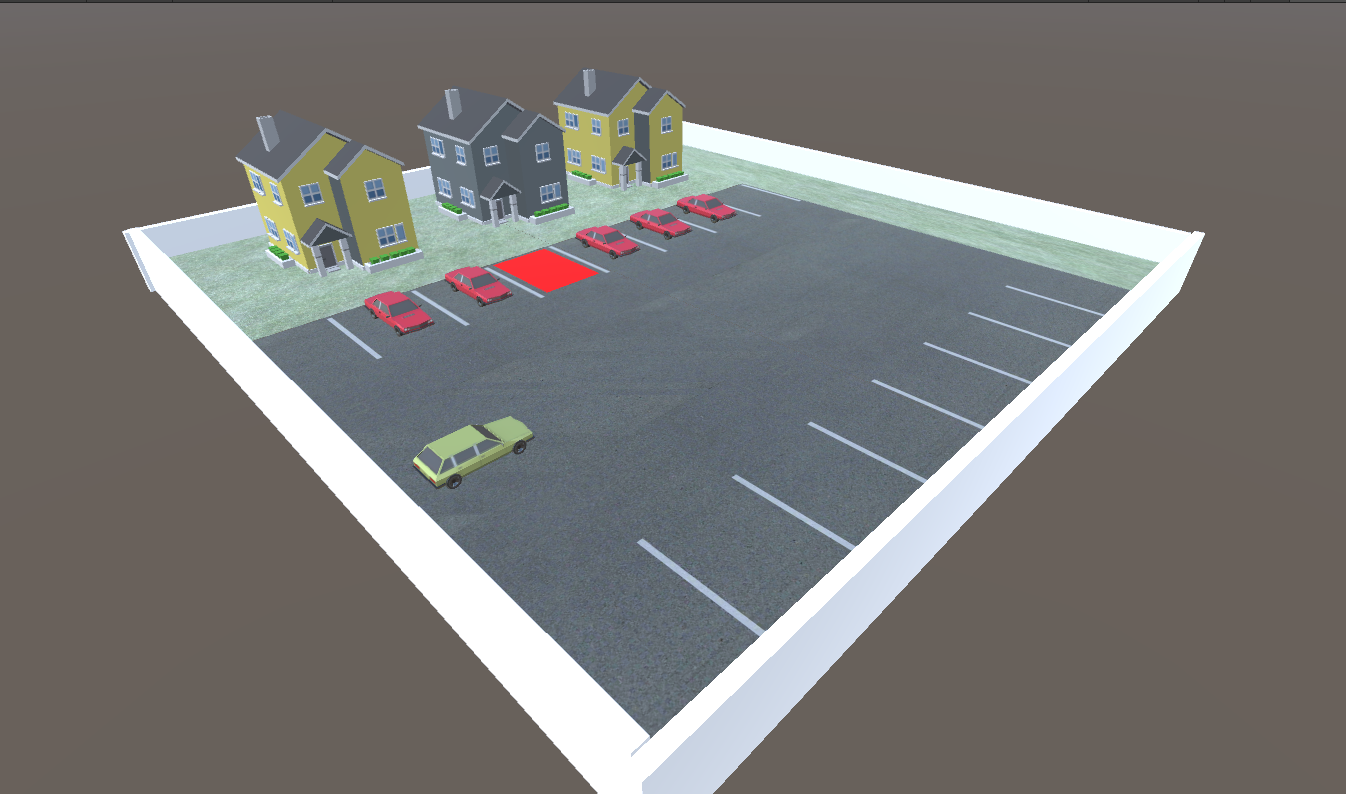
\includegraphics[scale=0.35]{environment}
    \caption{The parking lot environment in Unity Engine}
\end{figure}
The environment is a one floor parking scenario with a total of 16 parking spots. For this first experiment, the designated parking spot is fixed, as well as the other cars' positions. The car is considered to be parked when it stays within $0.6$ units from the spot for at least $0.5$ seconds. A unit in Unity is equivalent to 1 meter and the distance is computed from the center of the car to the center of the parking spot.

The agent is a low-polygon 3D car model equipped with a total of 24 depth sensors which can detect objects up to 5 units away.
\begin{figure}[H]
    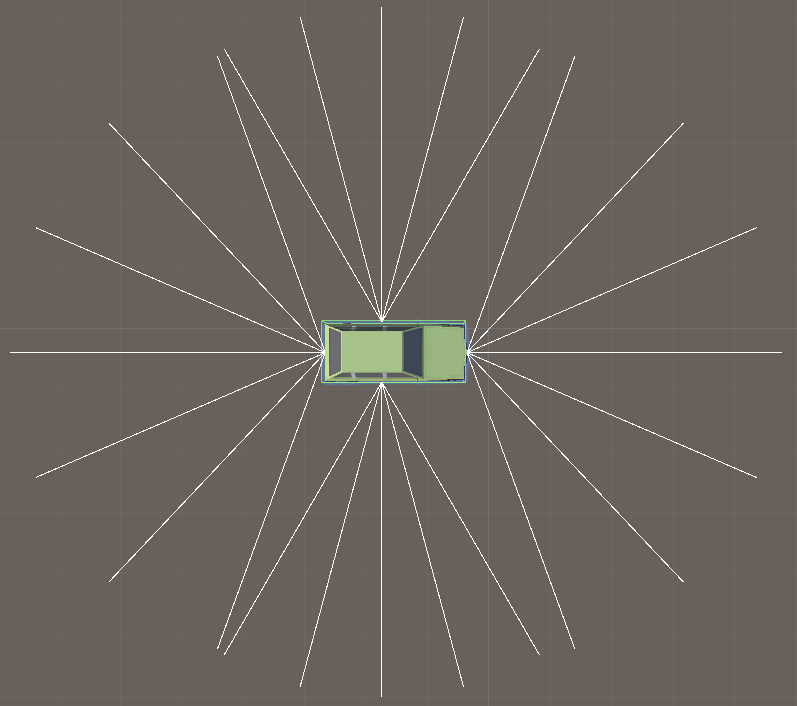
\includegraphics[scale=0.5]{car}
    \caption{The car (agent) and its sensors}
\end{figure}
The reward functions are described in the table below:
\begin{table}[H]
\begin{tabular}{|l|c|}
\hline \multicolumn{1}{|c|}{ Reward function } & Value \\
\hline Timeout & $-1000$ \\
\hline Parking successfully & $1000$ \\
\hline Parking successfully and sufficiently aligned & $5000$ \\
\hline Time & $-2$ per timestep \\
\hline Stopping & $-0.0002$ per timestep \\
\hline Collision & $-1$ \\
\hline Stay in collision & $-0.5$ per timestep \\
\hline Goal heading & $-1$ to $1$ per timestep, see below for details\\
\hline Goal distance & $-1$ to $1$ per timestep, see below for details\\
\hline
\end{tabular}
\caption{\label{tab:rewards}Reward functions for the agent.}
\end{table}
During the first few experimental runs, we tried multiple ways of encouraging the agent to get closer to the goal, but, of course, without actually telling the exact coordinates. Rewarding it for getting closer compared to the previous time step was our first successful attempt at teaching the agent to park at the designated spot, but the success rate was still rather low. The agent would often get stuck in a loop going back and forth and the episode would eventually end due to timeout.

With the intent of proving a better incentive for getting closer, we designed a custom curve to define the rewards the agent would get based on its distance from the parking spot.
\begin{figure}[H]
    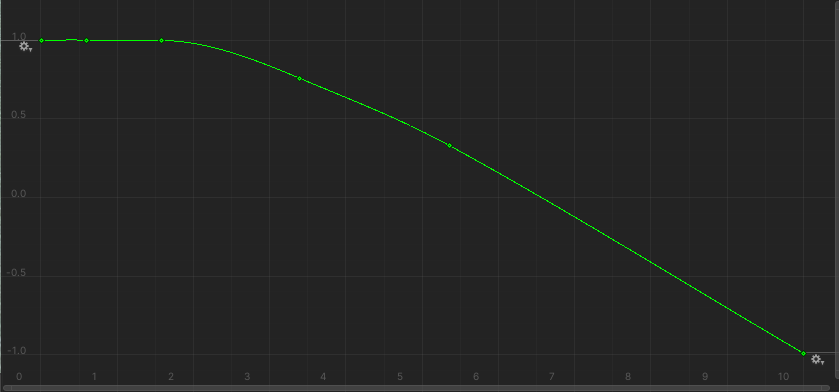
\includegraphics[width=\textwidth]{goal_reward_curve}
    \caption{The reward function for getting closer to the goal}
    \label{fig:goaldist}
\end{figure}
The $x$-axis ranges from $0$ to $10$ and represents the distance between the agent and the goal. The $y$-axis ranges from $-1$ to $1$ and increases as the agent gets closer to the spot. From the very first attempt, these reward functions showed very good results, with success rates above $50\%$. However, the agent would often park completely disaligned.

To seek further improvement, we also rewarded the agent at each time step based on whether it was heading towards the goal or not. The reward is the dot product between the vector pointing forward from the car and the vector pointing forward from the parking spot, such that the reward is $1$ when the agent and the parking spot are perfectly aligned and $-1$ when the agent is headed the complete opposite way. Note that this measure is invariant of distance. Adding this extra reward function not only increased the success rate to almost $100\%$, but also significantly decreased training time. Unfortunately, it hadn't solved the original issue.

As an second attempt, we added an extra criterion to define whether the agent is parked or not. If the dot product between the two vectors mentioned above is $\geq 0.9$ at the moment of parking, the reward of $1000$ is given and the episode ends. If the dot product is $\geq 0.97$ the reward is increased to $5000$. In angles, since both vectors are unitary, the dot product is simply the cosine between the two vectors, that is, the angle must be at most $45\degree$ to consider the agent parked and at most $\approx 25\degree$ to receive the bonus reward. In terms of training time and success rate, nothing has changed, but the agent would always park correctly and get the bonus once trained.

Lastly, we noted that the policy the model converged to was not always the same. One of these policies is what we actually intended to achieve - parking as aligned as possible and in the least time possible. The second is what we believe to be the optimal policy, since it yielded the most reward compared to the other - the agent would stop very close to the spot, in such a way to receive the maximum reward possible from both the alignment and distance criteria. The workaround was to increase the penalty at each time step, so that exploiting the rewards for distance and alignment would never be more beneficial than parking. After that, the model would always converge to the same policy, guaranteeing the result was reproducible.

The value of hyperparameters used and the results are presented below. 
\begin{table}[H]
    \begin{tabular}{|l|c|}
    \hline \multicolumn{1}{|c|}{ Hyperparameter } & Value \\
    \hline Divergence limit $\epsilon$ & $0.2$ \\
    \hline Exponential discount $\lambda$ & $0.95$ \\
    \hline Epochs & $3$ \\
    \hline Discount factor $\gamma$ & $0.99$ \\
    \hline Batch size & $2048$ \\
    \hline Buffer size & $20480$ \\
    \hline Learning rate $\alpha$ & $3 \cdot 10^{-4}$ \\
    \hline Number of layers & $2$ \\
    \hline Number of hiddens unit & $256$ \\
    \hline Time horizon & $512$ \\
    \hline Max step & $5\cdot 10^{7}$ \\
    \hline
    \end{tabular}
    \caption{\label{tab:hyperparameters}Hyperparameter configuration.}
    \end{table}
The values used are the suggested values for training continuous action spaces models by Unity ML-Agents official documentation. The only hyperparameters tweaked were the time horizon and the max step, to guarantee the agent would have enough time to explore the environment and to make sure we would have enough training steps to converge to a policy.
\begin{figure}[H]
    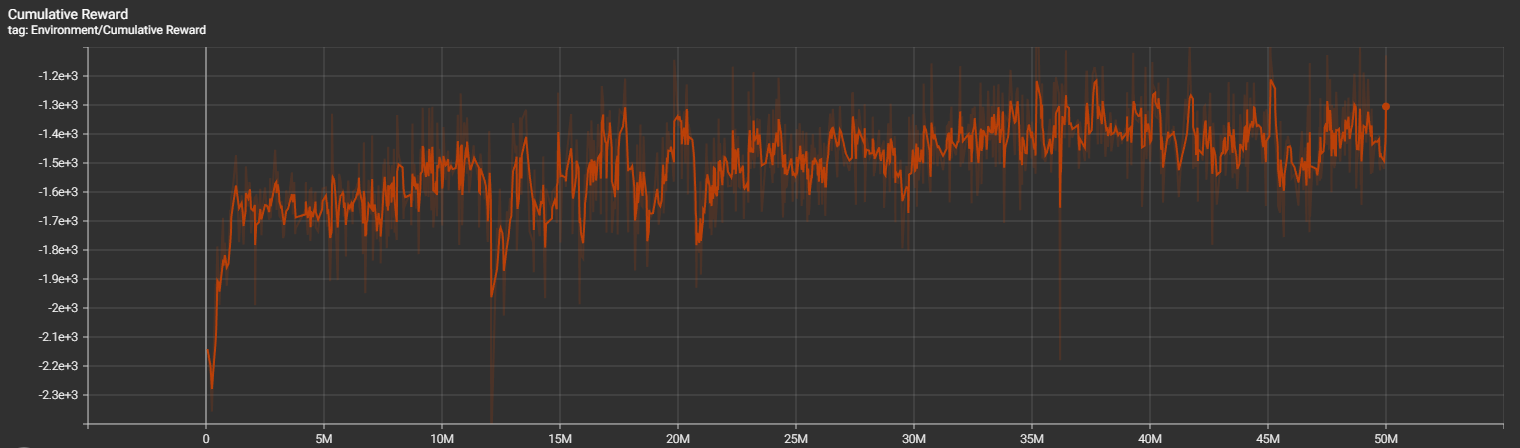
\includegraphics[width=\textwidth]{exp1/cumrewards}
    \caption{Cumulative rewards obtained by the agent during training.}
    \label{fig:cumrewards1}
\end{figure}
\begin{figure}[H]
    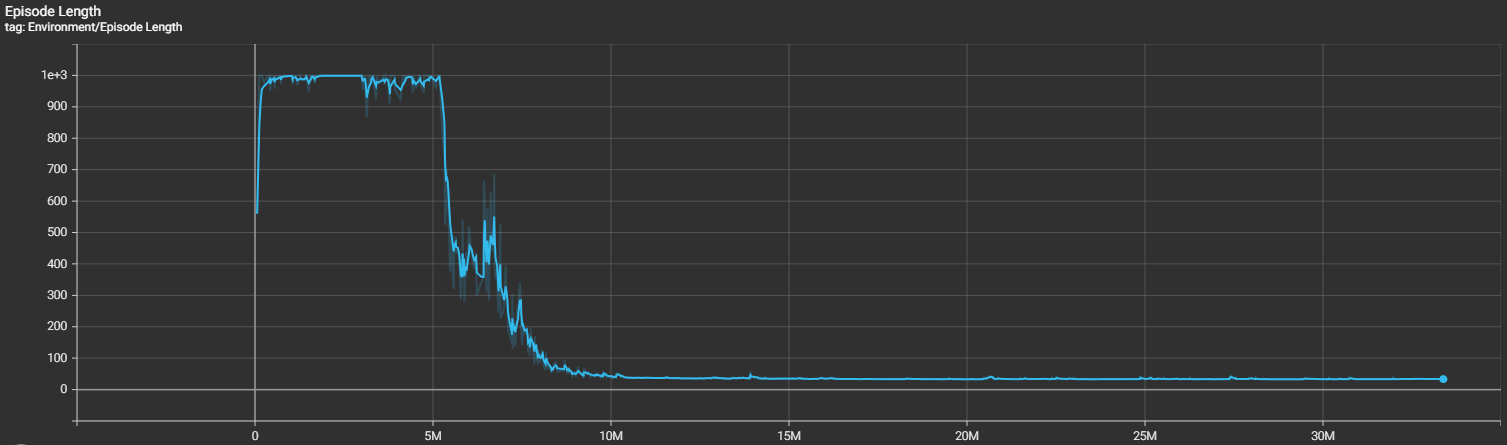
\includegraphics[width=\textwidth]{exp1/episodelength}
    \caption{Episode length during training.}
    \label{fig:episodelength1}
\end{figure}
\begin{figure}[H]
    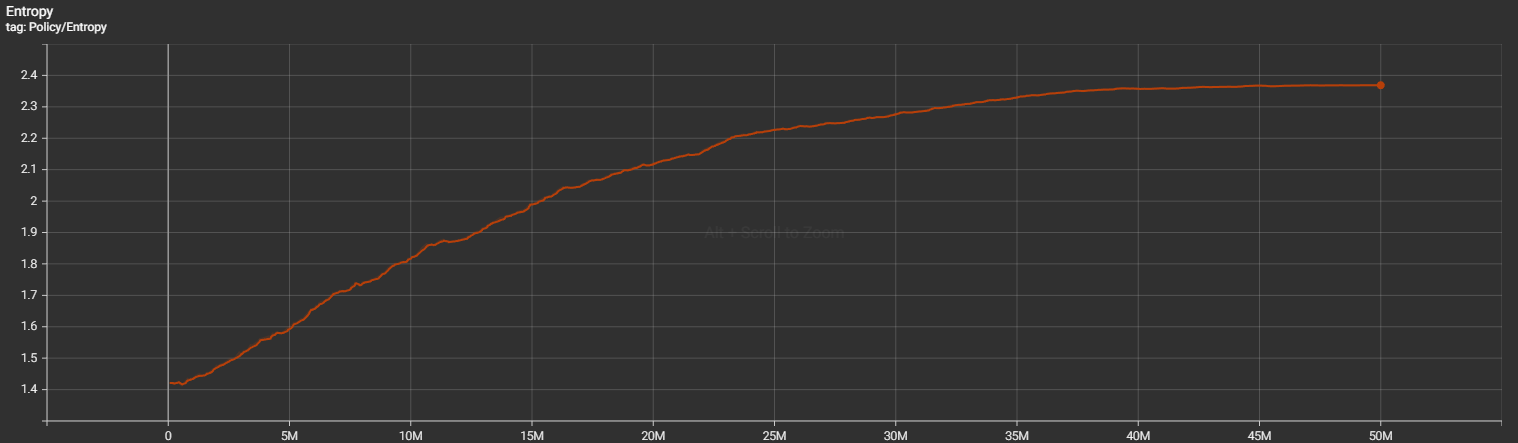
\includegraphics[width=\textwidth]{exp1/entropy}
    \caption{Entropy evolution during training.}
    \label{fig:entropy1}
\end{figure}
The behavior is completely random when training starts, but once it parks correctly for the first time, the agent is quick to learn what is to be achieved, and eventually learns how to do it in the least time possible. To summarize, the main challenges of this experiment was to provide enough incentive for the agent to reach the goal and working around eventual exploits the agent would find in our reward design that would make it not accomplish what was intended.
\section{Experiment 2: Randomized Car Position and Fixed Parking Spot}
\section{Experiment 3: Randomized Car and Parking Spot Positions}